\section{Platform}

\subsection{Overview}

This section describes the platform that was designed and built for the creation and curation of geospatial data, attempting to address the challenges described in \ref{challenges-of-crowdsourcing-geospatial-data}. The general workflow that describes what the platform is designed for is shown in Figure \ref{fig:workflow_0}.

\begin{figure}
	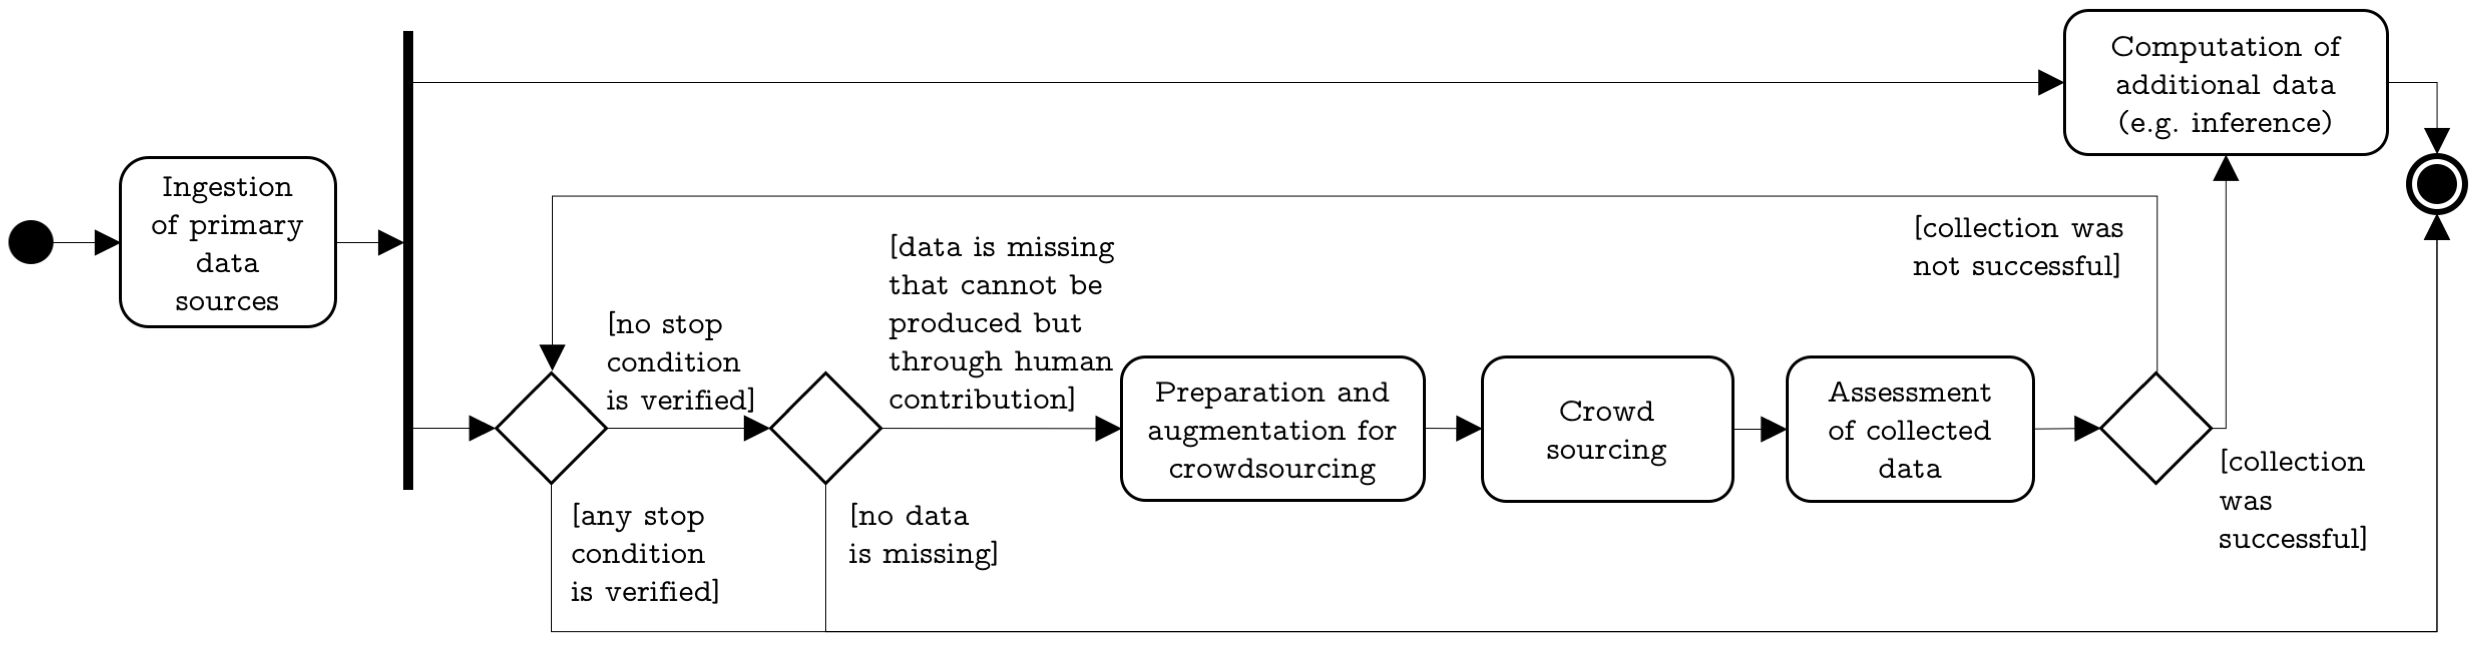
\includegraphics[width=1.0\textwidth]{workflow-0.png}
	\caption{General workflow}
	\label{fig:workflow_0}
\end{figure}

\subsection{Overall design principles}

In designing the platform, the design principles below were used as guidance:

\textbf{Support to human-machine workflows} The opportunity to exploit hybrid human-machine workflows was a key assumption in our research. The solution was required to automate as much as possible of the data creation / curation process while effectively integrating human components, from the crowdsourcing of part of the data to the administration of the process itself.

\textbf{Data re-use} Making the best possible use of pre-existing, reliable data was a key design driver, in particular to take advantage of the substantial volume of open data published in the UK over the last two-three years, and expecting a similar trend to be observable in many other countries in the upcoming years.

\textbf{Open source software} It was assumed that most original components required by the solution could be built using open source software only, also to preserve any available budget for the compensation of paid contributors to the crowdsourcing campaigns.

\textbf{Scalability and high availability} The solution was designed to be highly scalable and available - well beyond the needs of the experiments described later in this document - and suitable for real-world deployment.

\textbf{Versatility} The solution needed being versatile and suitable to support different workflows, input data sources and target output datasets. Despite the extensive literature, crowdsourcing in particular is still more of a craft than science and no design formula can assure success without experimentation. The design of the solution needed to support different forms of crowdsourcing across its many dimensions: paid contributors vs volunteers, results aggregation, quality assessment etc.

\subsection{Crowdsourcing component design principles}

The following is a high level description of the crowdsourcing component of the platform according to the dimensions presented in \cite{Wearethedata:2015uo}. The description is independent of the specific objective of the system. 

A general observation is that the crowdsourcing element was intentionally designed to explore characteristics that are far from what has been already extensively explored in VGI literature, particularly thanks to the opportunity to study the OpenStreetMap case. The hypothesis and ambition is that the finding of the research can be complementary to what can be achieved with VGI and enrich the set of tools available to the system designer.

\textbf{What is outsourced} The objective of the outsourcing activity is the production of original geospatial data or the correction / validation of pre-existing data, wherever the activity can be only performed by human agents. 

We use the term "geospatial data" in its wider connotation: data that relates to or is associated with a particular location. It can be about the geographic characteristics of a place (e.g. the topology of a street network), but also about facts associated to that place (e.g. how many trees in that street).

The activity typically translates into surveying the locations or examining imagery thereof and record observations (e.g. "how many trees can be seen from longitude x and latitude y?"), or, alternatively, amend some previous recording of the same (e.g. "can you confirm that there is a hospital in Vicarage Rd, Watford, Hertfordshire?"). 

To avoid the physical survey of the locations, participants examine publicly available imagery of the location. This is not uncommon, e.g. the OpenStreetMap website uses aerial imagery sourced from Microsoft Bing to let its contributors edit the topology of the streets\footnote{See \url{https://www.openstreetmap.org/edit}.}. The cost effectiveness of humans observers is expected to outperform machine learning, computer vision and automation in general for a few more years, particularly in observing imagery that are ambiguous [IT WOULD BE NICE TO QUOTE SOMEONE HERE].

\textbf{Who is the crowd} No specialised knowledge or skills are required, nor a connection to the places being surveyed. In VGI, though, contributors are often associated to the locations they work on, as it is both a driver for their motivation and direct knowledge of the place is occasionally necessary to assure the completeness of the data. The function of buildings or the location of mailboxes, for example, can't be inferred from observing OpenStreetMap's aerial imagery. Moreover, the first survey of new locations, e.g. new developments before they are visible on aerial imagery, are often made using specialised equipment, e.g. to record GPS tracks\footnote{E.g. the OpenStreetMap project advises against using conventional mobile phone GPS functionality, as it can be very difficult to work out the technical accuracy of a track. See \url{http://wiki.openstreetmap.org/wiki/Recording_GPS_tracks}.}.

The crowdsourcing task design intends to assure the contributors detachment from the locations.

\textbf{How are the task outsourced} Again, to explore different formulae than what is common in VGI, the crowdsourcing component focus is on implementing micro rather than macro tasks, and, definitely, microtasks cannot be burdened with the overhead typical of surveying in the real world, like planning a journey and travelling to the location and back, use equipment etc. 

Wherever possible, one's contribution is limited to max few minutes of work at the computer, the shorter the time required the better. Ideal tasks are closed- rather than open-ended and require no particular thought or focus. The participant has no visibility of the workflow she is part of: the volume of effort spent in preparing the data, aggregating the responses, assessing their accuracy etc. 

\textbf{Why do people contribute} In VGI, crowds are made of intrinsically motivated volunteers: open data advocates, geospatial practitioners and individuals who are passionate about geography in general [SOME REFERENCE]. Our contributors are oblivious of the the context of the project, have no personal connection to the locations being surveyed, and likely are unaware of and find no motivation in contributing to the "cause" of open data in general. They perform their tasks driven merely by the financial reward. This is typically the crowd that can be recruited through mainstream crowdwork platforms such as Amazon Mechanical Turk and Crowdflower. 

\subsection{Implementation}

\subsubsection{Overview} \leavevmode \\ %% Why is this necessary to get a new line?

From the platform owner point of view, the system is made of:

\begin{enumerate}
    \item A set of tools to ingest the primary data sources into a reference database.
    \item A set of tools to process the ingested data and derive new / enhanced data computationally, e.g. through statistical inference.
    \item A set of templates to configure the crowdsourcing platform of choice - e.g. Amazon Mechanical Turk or CrowdFlower - and set up the interface the participants use to contribute.
    \item A set of tools to iteratively (i) identify what the highest priority gaps in the reference and derived data are, (ii) load data into the crowdsourcing platform accordingly, to enable the collection of what is missing and (iii) evaluate the crowd's output, until a stop condition is verified, e.g. the data was successfully collected and at the target level of quality, or, in the case of paid crowdsourcing all budget has been spent.
    \item A set of tools to consolidate the original, derived and crowdsourced data in one consistent dataset.
\end{enumerate}

From the participant point of view, the solution presents itself simply as a task hosted on their crowdsourcing platform of choice. The task web page offers interactive maps and a panoramic views of one or more locations to survey, and a form the participant will use to submit her observations, as shown in \ref{fig:virtual-survey-tool-01}. 

At the top of the page, for contributors who are new to the task, instructions are given, possibly enhanced by a video used to illustrate the interactive features of the map and panoramic view, as in \ref{fig:virtual-survey-tool-02}.

\begin{figure}[!ht]
    \begin{floatrow}
        \ffigbox{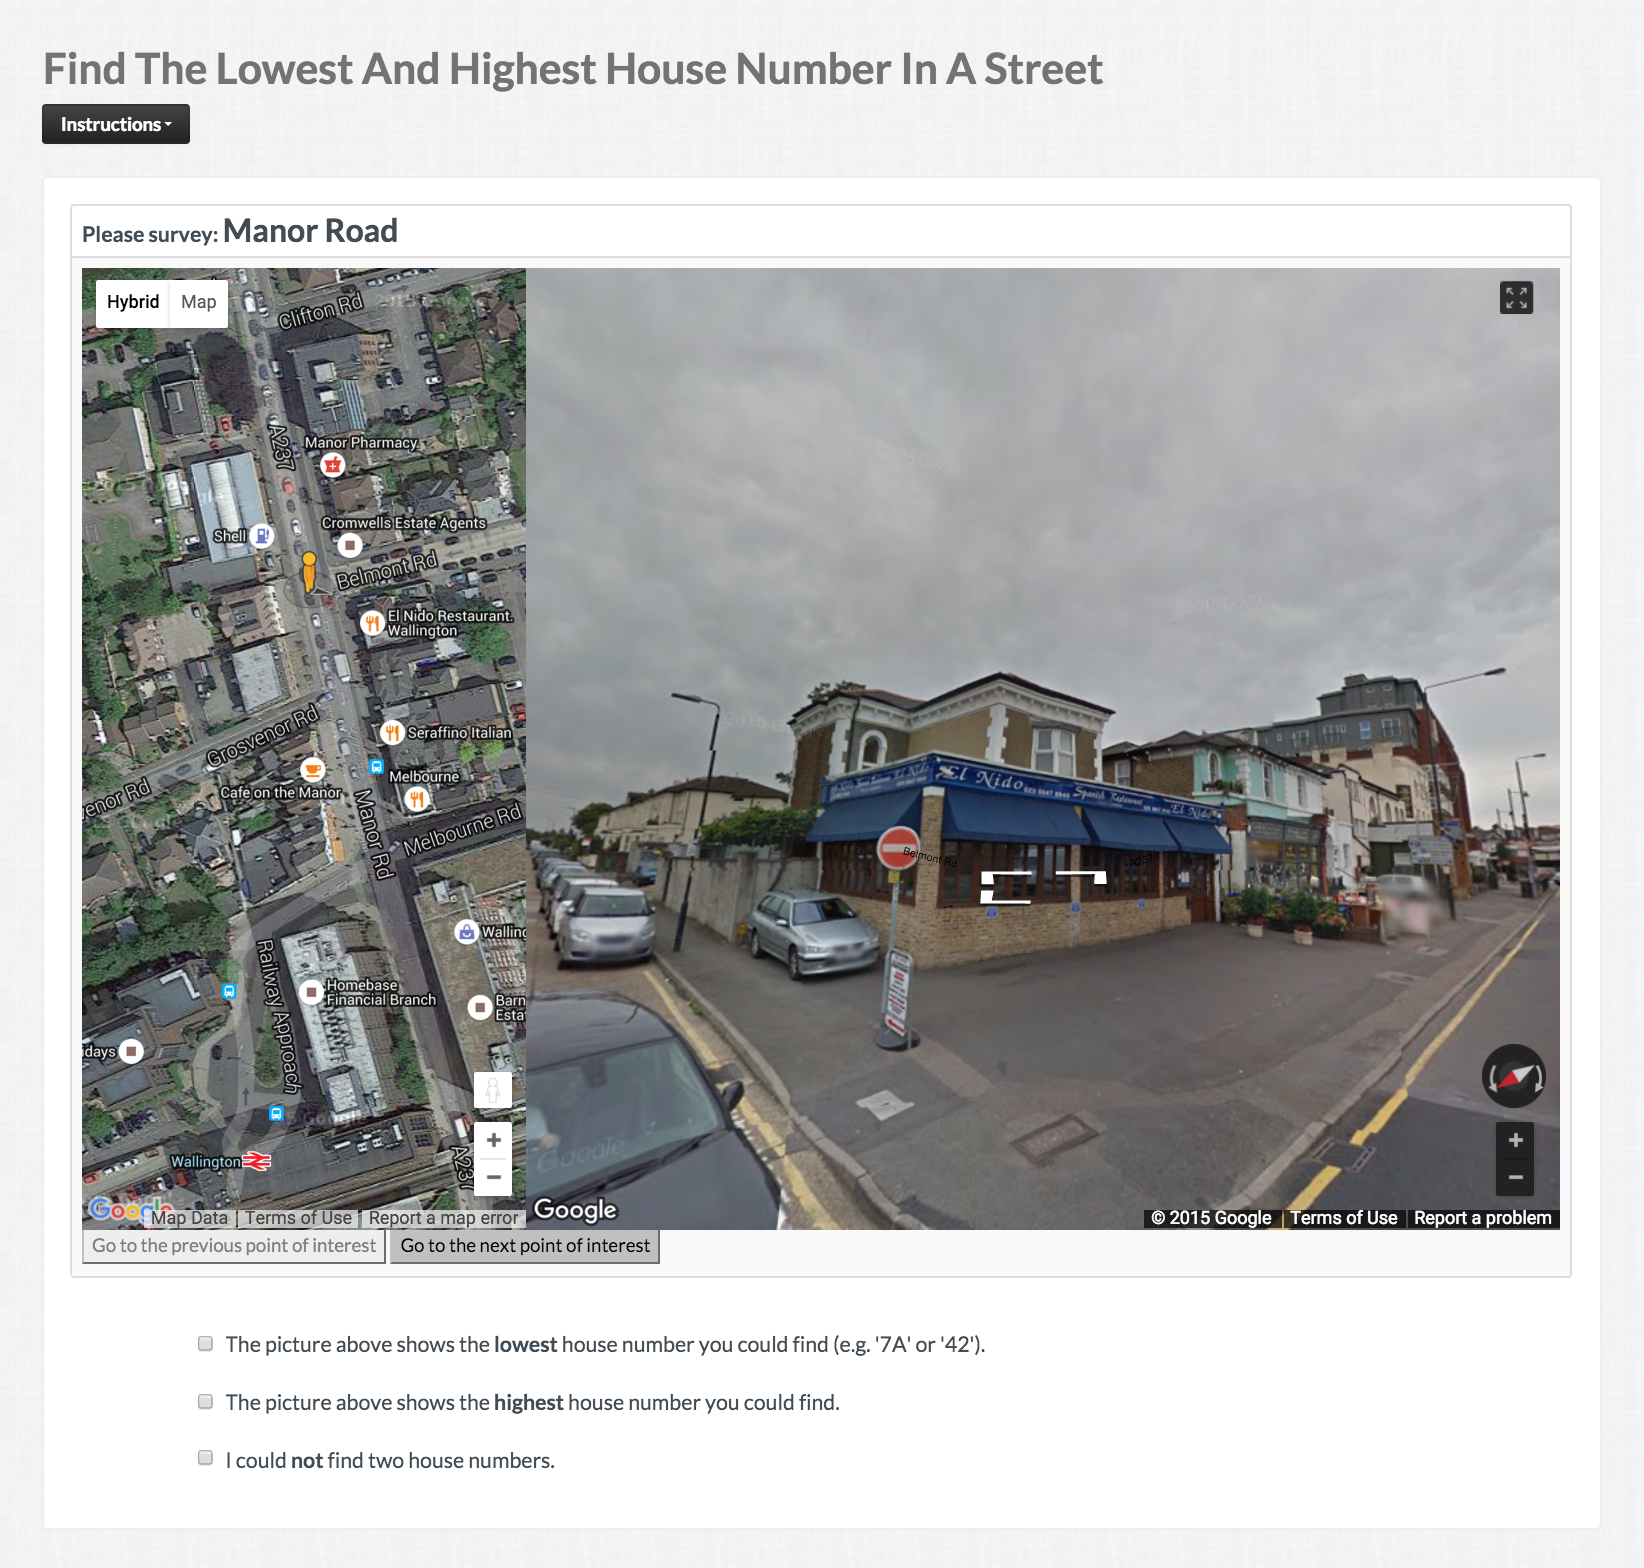
\includegraphics[width=0.45\textwidth]{virtual-survey-tool-01.png}}{\caption{The task section of the web page, offering the Google Maps and Street View panes and the form participants use to submit their observation.}\label{fig:virtual-survey-tool-01}}
        \ffigbox{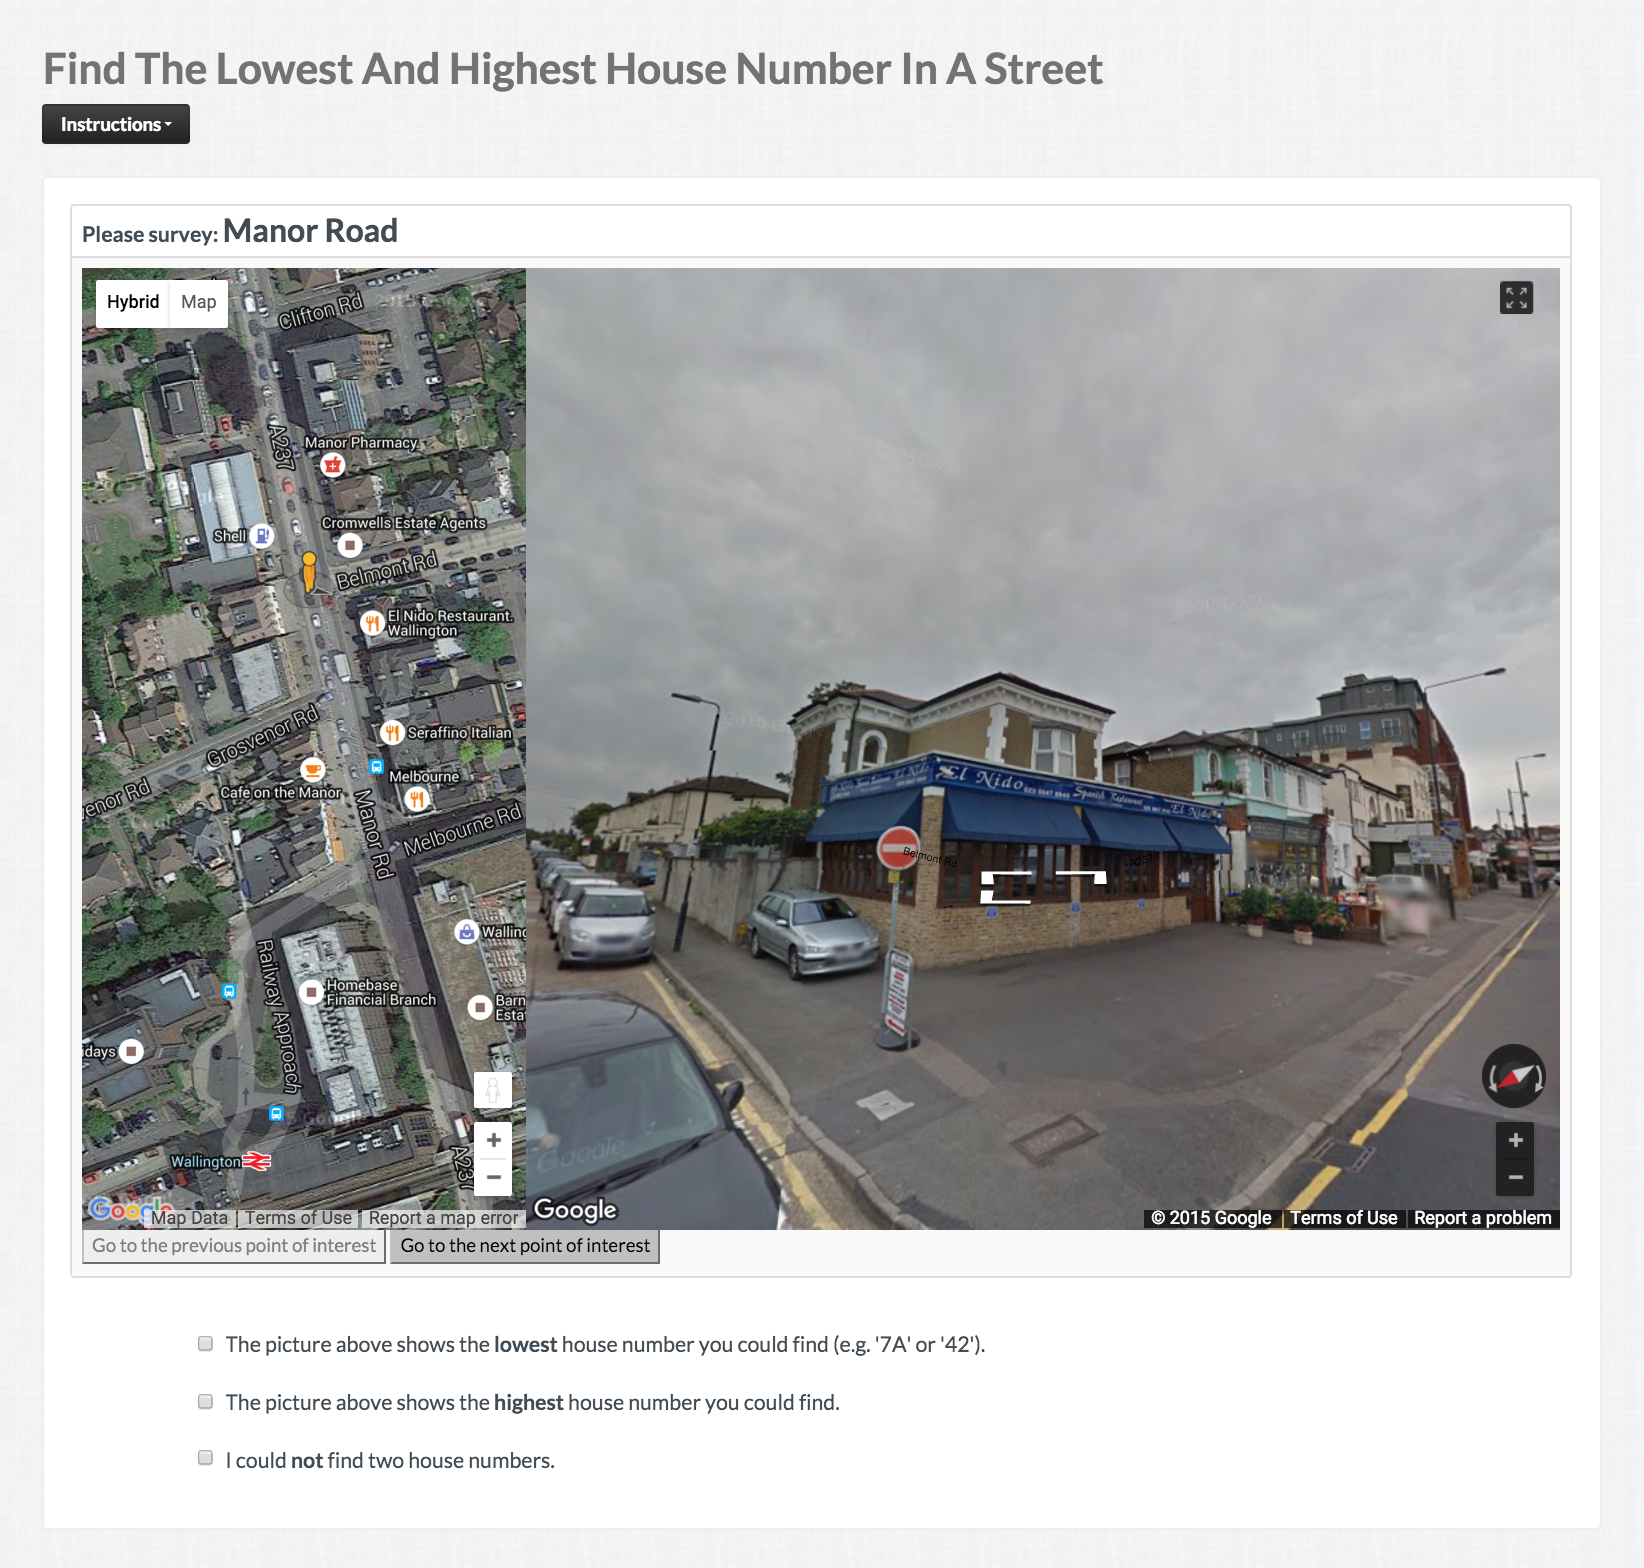
\includegraphics[width=0.45\textwidth]{virtual-survey-tool-01.png}}{\caption{The instruction section of the web page, embedding a video with the instructions.}\label{fig:virtual-survey-tool-02}}
   \end{floatrow}
\end{figure}


\subsubsection{Components} \leavevmode \\ %% Why is this necessary to get a new line?

\textbf{CrowdFlower} CrowdFlower was chosen as the crowdsourcing platform. It is a Software-as-a-Service platform specialised in hosting data-centred microtasks for volunteer or paid participants. Clients who accept that their data could be re-published as open data by CrowdFlower may access the service under the "Data for Everyone" plan, that has no costs but for the compensation to the paid participants and a 20\% commission. The service is available both through a templating system called "CrowdFlower Markup Language" (or "CML") that can be customised by using CrowdFlower's web-based tools, or through APIs. 

When using CML, the options available to implement a crowdsourcing model - such as how Worker accuracy is assessed or how results are aggregated - are limited by the functionality supported by the system\footnote{For example, CrowdFlower calculates the Workers' agreement simply as the \% of participants who expressed the majority vote, and tasks can be stopped automatically when a target agreement \% is achieved. If one wanted to use a stronger statistical tool to calculate agreement, such as Fleiss' Kappa, that automation cannot be used and the calculation must take place outside of the system.}. In order not to introduce additional components in the system and maximise scalability and high availability, it was decided to rely on CML only and work around its limitations by performing some of the tasks outside of CrowdFlower, e.g. results aggregation. 

\textbf{Google Maps} Google Maps is a Software-as-a-Service mapping service for the web and mobile devices, made available by Google to the public for free within the limitations of some terms of service. It offers satellite and aerial imagery, maps, interactive panoramic views of streets ("Street View") and the respective metadata through APIs. Many of its services can be embedded in third party websites and customised using client-side JavaScript, hence making it very suitable to be integrated with CrowdFlower or any other template-based content management systems. 

It was decided to use Google's mapping services for the prototype as the team had already experience of programming with it. Other equivalent services could have been used as well, e.g. Microsoft's Bing Maps.

\textbf{YouTube} YouTube is a video publishing platform owned by Google. As for Google Maps, videos can be embedded in third party websites, hence YouTube is suitable to be integrated in CrowdFlower's CML templates. The platform uses YouTube to offer participants the instructions video.  

\textbf{PostgreSQL + PostGIS} The PostgreSQL relational database\footnote{See \url{http://www.postgresql.org/}.} running the PostGIS spatial extender \footnote{See \url{http://postgis.net/}.} was chosen as the main data repository for the platform. All geospatial data is converted from its original format (CSV, ESRI Shapefile etc.) to PostGIS' native geospatial types to be consistent across all sources and enabling spatial and geographic querying. When needed, QGIS \footnote{See \url{http://www.qgis.org/}.} can be used to quickly visualise the data on maps, e.g. for inspection and debugging.

\textbf{Scripting} Bash, NodeJS and PostgreSQL SQL scripting are used to glue all components together wherever automation is possible across the many stages of:  

\subsubsection{Legal aspects}

The choices made in designing an implementing the platform can have legal implications that need to be taken into account, in particular if the data that is the result of the process is intended to be published under an open licence.

It is outside of the scope of this paper to examine this in detail, although it is useful to present, in the following, some of the issues to consider.

\textbf{Personal data and privacy implications.} According to EU Data Protection Directive (95/46/EC\footnote{See \url{http://eur-lex.europa.eu/LexUriServ/LexUriServ.do?uri=CELEX:31995L0046:en:HTML}.} some geospatial data such as addresses can be considered "personal data" even when it is not associated to information about {\it who} lives at those locations, as it is "information relating to an identified or {\it identifiable} natural person" (no italics in the original). The directive describes a framework of good practices for member states to make into law that we would need to comply with.
	
\textbf{Imagery terms and conditions} Google Maps' terms of service \footnote{See \url{https://www.google.com/intl/en-GB_US/help/terms_maps.html}.} specify a restriction on producing "derivative works of the Content or any part thereof". Moreover, and more specifically, they also include a restriction on using the services to create "a database of places or other local listings information". It can be argued that observing a map or the pictures of a street does not constitute "derivative work". In any case, it is advisable that - before deploying the platform to real-world applications - the mapping services provider is informed and licensing clarified. This is what OpenStreetMap did to integrate Bing imagery\footnote{See \url{http://wiki.openstreetmap.org/wiki/Bing#Bing_Aerial_Imagery}, last accessed 2 January 2016.}.
